\section{Results}

\begin{figure}[t]
\centering
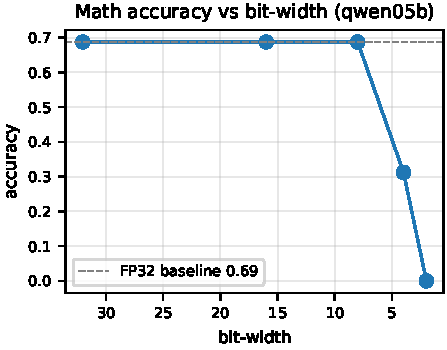
\includegraphics[width=\columnwidth]{figures/acc_vs_bits_qwenZeroFiveb.pdf}
\caption{Math accuracy vs.\ bit-width on Qwen2.5-0.5B (synthetic arithmetic
benchmark). The dashed line is the FP32 baseline.}
\label{fig:acc-bits}
\end{figure}

\begin{figure}[t]
\centering
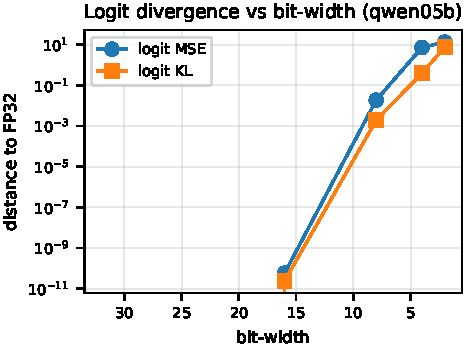
\includegraphics[width=\columnwidth]{figures/mse_vs_bits_qwenZeroFiveb.pdf}
\caption{Logit MSE and KL divergence to the FP32 reference as a function
of bit-width. Both metrics span many orders of magnitude across the sweep,
consistent with the expected scaling law of weight perturbation
$\sim 2^{-b}$.}
\label{fig:mse-bits}
\end{figure}

\paragraph{Bit-width sweep.} At 4-bit, accuracy is
$\qwenZeroFivebAccBitsFour$ and logit MSE $\qwenZeroFivebMSEBitsFour$;
at 2-bit (ternary), accuracy collapses to
$\qwenZeroFivebAccBitsTwo$ and logit MSE rises to
$\qwenZeroFivebMSEBitsTwo$. The qualitative ordering
$\text{MSE}(32)<\text{MSE}(16)<\text{MSE}(8)<\text{MSE}(4)<\text{MSE}(2)$
holds without exception and over several decades on the logarithmic
scale of Figure~\ref{fig:mse-bits}.

\begin{figure}[t]
\centering
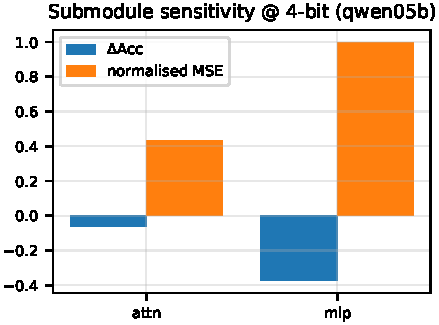
\includegraphics[width=\columnwidth]{figures/sensitivity_qwenZeroFiveb.pdf}
\caption{Submodule sensitivity at 4-bit. Quantizing only attention weights
yields $\Delta\text{Acc}=\qwenZeroFivebSensAttnDeltaAcc$ and logit
MSE $\qwenZeroFivebSensAttnMSE$; quantizing only the MLP yields
$\Delta\text{Acc}=\qwenZeroFivebSensMlpDeltaAcc$ and logit MSE
$\qwenZeroFivebSensMlpMSE$.}
\label{fig:sens}
\end{figure}

\paragraph{Submodule asymmetry.} Figure~\ref{fig:sens} shows that attention
and feed-forward weights contribute asymmetrically. The submodule whose
quantization induces a larger logit MSE is the natural candidate to
\emph{exclude} from aggressive quantization in a mixed-precision schedule.
The proposed "reasoning-aware" mixed-precision recipe is: keep the more
sensitive submodule at FP16 (or INT8) and quantize the rest to INT4. The
GPU configuration extends this analysis to GSM8K and reports the Pareto
curve.
